\documentclass {article}

\usepackage[none]{hyphenat}
\usepackage[utf8]{inputenc}
\usepackage[english]{babel}
\usepackage[document]{ragged2e}
\usepackage {hyperref}
\usepackage {float}
\usepackage {graphicx}
\usepackage {fullpage}


\hypersetup {
	colorlinks = true,
	linkcolor = blue,
	urlcolor = cyan,
}

\title {Referencing the Combinatorics DLL}
\author {Anthony Morast}
\date {\today}

\begin{document}

\maketitle

\section {Referencing the DLL in a Visual Studio Project}
This section will go over how to download the combinatorics dll and add it as a reference to a Visual Studio project. This section will not cover beginning using the classes within the dll, that
will be covered in subsequent sections. \\

\vspace{5mm}

Note that this dll can be used outside of Microsoft Visual Studio. If you are using some other compiler/integrated development environment add the dll as you wish. This document focuses on Visual Studio because C\# is a .NET language and, until recently, has little support on other platforms or in other environments. \\

\vspace{5mm}

The following steps will show how to get the the combinatorics DLL\\ downloaded to your machine:
\begin{enumerate}
	\item Go to the GitHub repository \href{https://github.com/anthonyam12/CombinatoricsLibrary}{here}.
	\item Near the top center of the screen there will be a \textit{release} link.
	\begin{figure}[H]
		\centerline{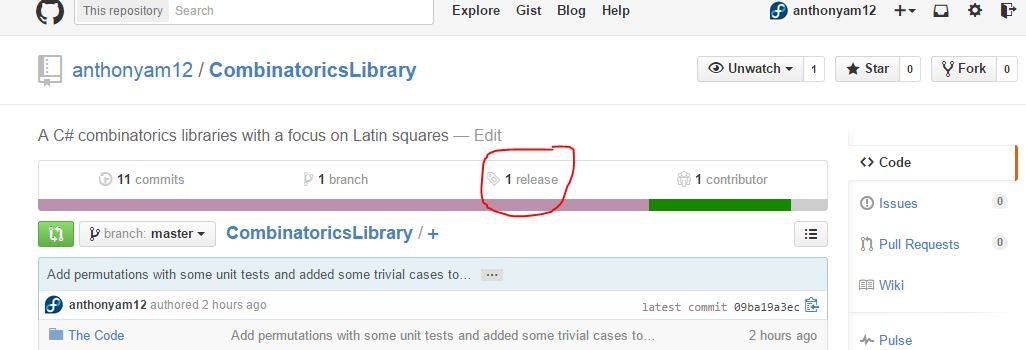
\includegraphics[width=175mm, scale=1]{ReleaseLink.jpg}}
	\end{figure}
	\item This will bring up a web page that allows you to download the source code (which includes the dll) or just the dll, choose whichever is best for your situation.
	\item Here is how to find the dll depending on which method you choose:
	\begin {enumerate}
		\item If you choose to download the source code along with the dll, simply unzip the package and traverse to the \textit{TheDLL(s)andHowTos} folder to find the dll.
		\item If you choose to download the dll alone, then it should be floating around somewhere in your downloads folder.
	\end {enumerate}
	\item Regardless of how you obtain the dll keep track of its location so you can add it to your C\# application.
	\begin {enumerate}
		\item I recommend copying the dll to the folder of the project in which you wish to use the combinatorics library so that it will be packaged with the solution.\\
 		\vspace{2mm}
		This will avoid missing reference errors if the dll is removed from the downloads folder or if the C\# project is moved between machines. 
	\end 	{enumerate}
	\item Now that the dll is downloaded and you (hopefully) have access to its location, it's time to fire up the C\# project for which the dll is required. 
	\item Once inside Visual Studio open the project within the solution explorer where the dll will be referenced.
	\begin {enumerate}
		\item If you are having trouble finding the solution explorer it can be accessed via the \textit{VIEW} tab on the tool bar, this will produce a drop down menu which, for me, 				solution explorer is at the top. \\ \vspace{2mm} Alternatively, you can use the keyboard shortcut \textit{CTRL+ALT+L} to open the Solution Explorer.
	\end {enumerate}
	\item Here right click on \textit{References} and select \textit{Add Reference...}.
	\begin{figure}[H]
		\centerline{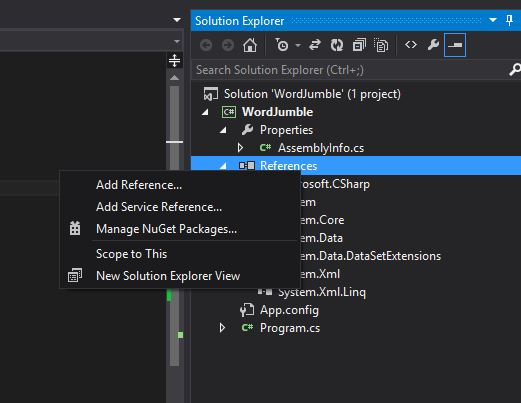
\includegraphics[width=70mm, height=80mm]{AddReference.JPG}}
	\end {figure}
	\item This will produce a dialog that has many options for adding assemblies, we will choose browse.
	\begin{figure}[H]
		\centerline{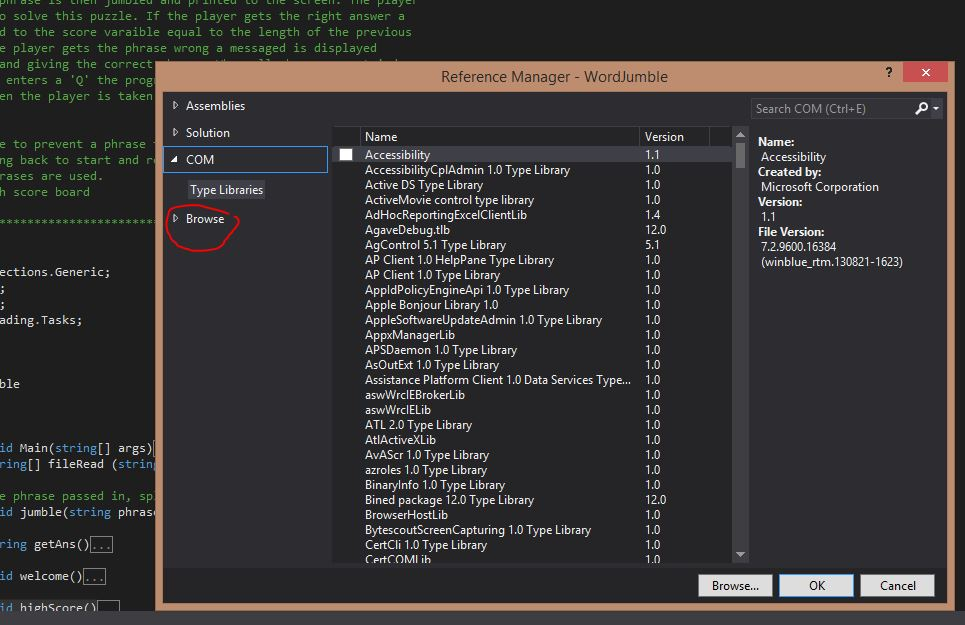
\includegraphics[width=130mm, height=55mm]{ReferenceDialog.JPG}}
	\end {figure}
	\item Clicking \textit{Browse...} in the lower right corner of this dialog will produce another dialog which allows you to choose a dll from your file system.
	\item Traverse to the location of the dll downloaded from GitHub, select it, and click \textit{Add}, again in the lower right corner. 
	\item The reference to the Combinatorics Library is now in your project! To begin using it add \\ \textit{\textcolor{blue}{using} CombinatoricsLibrary} at the top of the C\# file in which you wish to use it.
\end{enumerate}

\vspace{10mm}

This should get you up and running with this library. In the following tutorials I will cover some of the functionality, basic and advanced, of the methods and classes in this library. \\

\vspace{5mm}

If you want to jump right in to using this library without reading through tutorials there is also documentation on the individual classes in functions in the \textit{TheCode} folder and on the project's Wiki.

\end{document}